\listoftodos
34\_40 Tonnen
7m
16 pro tag





\chapter{Grundlagen}
\label{chap:Grundlagen}

	\section{TODO GRUNDALGENDETAIL}
	\label{sec:TODOGrundlagenDetail}
	\todo{notwendige klassische Grundlagen definieren} 
		Stacked Convolutional Auto-Encoders Stacked Convolutional Auto-Encoders for
		Hierarchical Feature Extraction
		Jonathan Masci, Ueli Meier, Dan Ciresan, and Jurgen Schmidhuber
		Istituto Dalle Molle di Studi sullIntelligenza Artificiale (IDSIA)
		Lugano, Switzerland
		{jonathan,ueli,dan,juergen}@idsia.ch
		
 			- layerwise pretrain {Greedy Layer-Wise Training of Deep Networks}
		- repraesentationen
		- transferlearning
	\section{Bibliotheken und Werkzeuge}
	\label{sec:BibliothekenundWerkzeuge}
	Für den Praktischen Teil der Abschlussarbeit wurde als Entwicklungsumgebung Cnvrg \cite{cnvrg.io.} genutzt. Cnvrg.io ist eine "full-stack Data Science Platform" welche Werkzeuge für die Erstellung, Verwaltung, Bereitstellung und Automatisierung von maschinellem Lernen bereitstellt. Cnvrg erlaubt es Arbeitsbereiche mittels Containern zu erstellen. Die Container können dabei auf Maschinen in Azure[] zugreifen. Für die Experimente wurde ein vorgefertiger Container mit einer tesla-k80 \cite{Nvidia.2020}, fünf CPUs und 49 GB Arbeitspeicher genutzt. 

	Für die Entwicklung wurden insbesondere Python \cite{PythonSoftwareFoundation.2020}, Jupyter Notebooks \cite{ProjectJupyter} und das Framework Tensorflow \cite{MartinAbadi.2015}  genutzt. Die wichtigsten Bibliotheken für die Arbeit sind Keras \cite{Chollet.2015} , Numpy \cite{Oliphant.2006} , Matplotlib \cite{Hunter.2007} , scikit-learn \cite{Pedregosa.2011} , ConfigSpace \cite{Lindauer.8162019} , Bayesian Optimization and Hyperband \cite{StefanFalkner.2018} . 
	
	Insbesondere für die Visualisierung von Embeddings wurde das Werkzeug PSIORI Visualizer erweitert und eingesetzt. Der Visualizer erlaubt es Daten in 3D darzustellen, von verschiedenen Blickwinkel und Zoomstufen zu betrachten, zu Filtern und mit zusätzlichen Informationen zu versehen. 
	\begin{figure}[h]
		\centering
		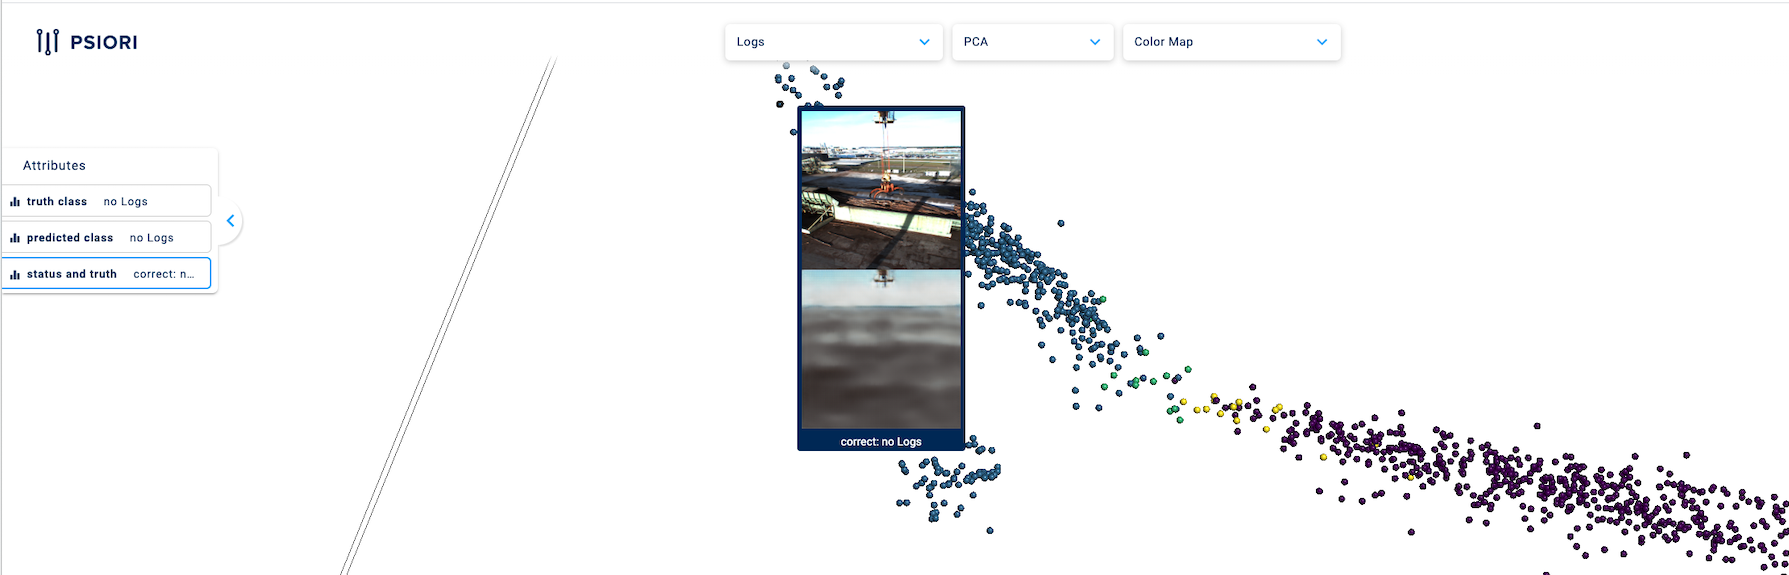
\includegraphics[width=1\textwidth, center]{bilder/Grundlagen/Example_Visualizer.png}
		\caption[Beispiel PSIORI Visualizer]{Beispiel PSIORI Visualizer}
		\label{img:ExampleVisualizer}
	\end{figure}  
	Die Abbildung \ref{img:ExampleVisualizer} zeigt einen Screenshot einer Visualisierung eines  Embeddings. Als zusätzliche Information sind die Datenpunkte entsprechend einer Klassifikation in True-Positiv, True-Negativ, False-Negativ und False-Positiv eingefärbt. Über einen Datenpunkt kann mit der Maus geschwebt werde,n um ein Bild anzuzeigen. Diese Funktion wurde insbesondere zum Anzeigen eines Orginalbildes und ihrer Rekonstruktion mittels Autoencoder genutzt. 
	
	Kern des praktischen Teils der Arbeit ist das Framework  Psipy \cite{PSIORIGmbH.2019}.	
	Psipy ist ein Python-Framework für Maschinelles Lernen welches von PSIORI selbst entwickelte Modelle zusammenfasst und eine einheitliche API zu Verfügung stellt. Diese API ist an die API des verbreiteten Frameworks scikit-learn angelehnt und die Modelle aus scikit-learn können in das von Framework eingebunden werden. Das Framework ermöglicht außerdem das Einbinden von Modellen basierend auf TensorFlow.

	
	In den nachfolgenden Abschnitten werden die wichtigsten Module des Frameworks vorgestellt. Diese Module wurden beim erstellen der neuen Module genutzt.
	
	 \paragraph{saveable.py} Das Modul Saveable bietet Kernfunktionalität zum Speichern und Laden von Klassen. Dabei werden verscheidene Arten von Modellen welche diverse Bibliotheken nutzen können auf eine einheitliche Art und Weise gespeichert. 

	\paragraph{autoencoder.py} Das Modul Autoencoder enthält die drei Klassen StackedAutoencoder, FullyConnectedAutoencoder und ConvolutionalAutoencoder. Der StackedAutoencoder wird als Vaterklasse für die anderen beiden Klassen genutzt. Im Konstruktor werden Methoden aufgerufe,n welche in den Kindklassen ausprogrammiert sind. Dabei wird ein Keras-Modell für einen Encoder und Decoder enstprechend von Parametern  erstellt. Als weitere wichtigen Methoden gibt es die Methode pretrain und fit. Mittels pretrain werden die Schichten eines symmetrischer Autoencoder von aussen nach innen wie in 	\todo{Quelle Autoencoder pretrain} Greedy Layer-Wise Training of Deep Networks  vortrainiert. Die Auswahl der Schichten erfolgt wieder in den Kindklassen.
	In der fit-Methode wird nach einigen Prüfungen die Methode fit() 	\todo{Quelle fit Keras}	[fit Keras] des Kerasmodells aufgerufen. In Abbildung \ref{img:KlassendiagrammConvolutionalAutoencoder} ist das Klassendiagramm mit den öffnetlichen Methoden des ConvolutionalAutoencoder dargestellt. 
	\begin{figure}[h]
		\centering
		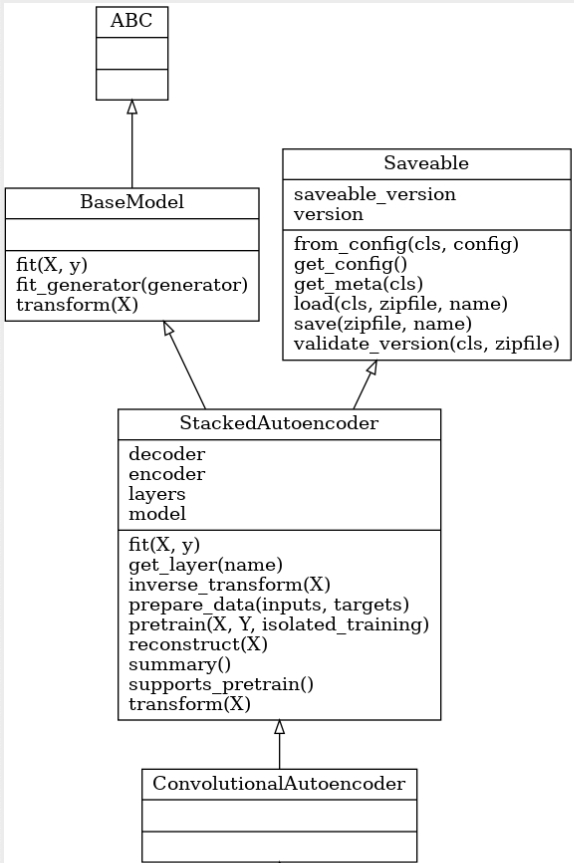
\includegraphics[width=0.5\textwidth, center]{bilder/Klassendiagramme/klassendiagramm_public_cae.png}
		\caption[Klassendiagramm ConvolutionalAutoencoder]{Klassendiagramm ConvolutionalAutoencoder}
		\label{img:KlassendiagrammConvolutionalAutoencoder}
	\end{figure}  
	
	\paragraph{hyperparameter\_mixin.py}  Hyperparameter\_mixin wird zum Standardisierten ablegen von Hyperparametern für AutoML Klassen genutzt. Auf die Hyperaparameter kann anschließend einheitlich zugegriffen werden.
	
	\section{Einordnung und bestehende Systeme}
	\label{sec:BestehendesSystem}
	Die Bilddaten und Aufgabenstellungen der neuronalen Netzwerke sind in die Problemstellungen des Autocrane-Projekts von PSIORI einzuordnen. Es sind also echte Datensätze und echte Problemstellungen, wobei die gezeigten Aufgabenstellungen und Modelle nicht zwingend in dem Autocrane-Projekt zum Einsatz kommen. Das Autocrane-Projekt ist ein laufendes Projekt, welches das Ziel hat, einen feststehenden Rundlaufkran vollautomatischen zu steuern. In Abbildung \ref{img:CircularCrane} ist ein Rundlaufkran abgebildet. Dieser Kran wird in einer holzverarbeitenden Anlage zum Befüllen eines Fülltrichters eingesetzt. Dabei sind insbesondere drei Anwendungsfälle interessant. Die Baumstämme werden mittels LKW angeliefert und müssen nach vorgegebenen Regeln (z. B. Ausrichtung, freier Lagerplatz) als Holzstapel gelagert werden. Der Fülltrichter muss mit Holz aus den Holzstapeln oder vom LKW aus befüllt werden. Es ergeben sich also Aufgabenstellungen wie Greifer-Erkennung, Baumstamm-Erkennung, LKW-Erkennung, Strategien für das entladen und aufbewahren der Baumstämme und vieles mehr. \cite{PSIORIGmbH.2020}
	\begin{figure}[h]
		\centering
		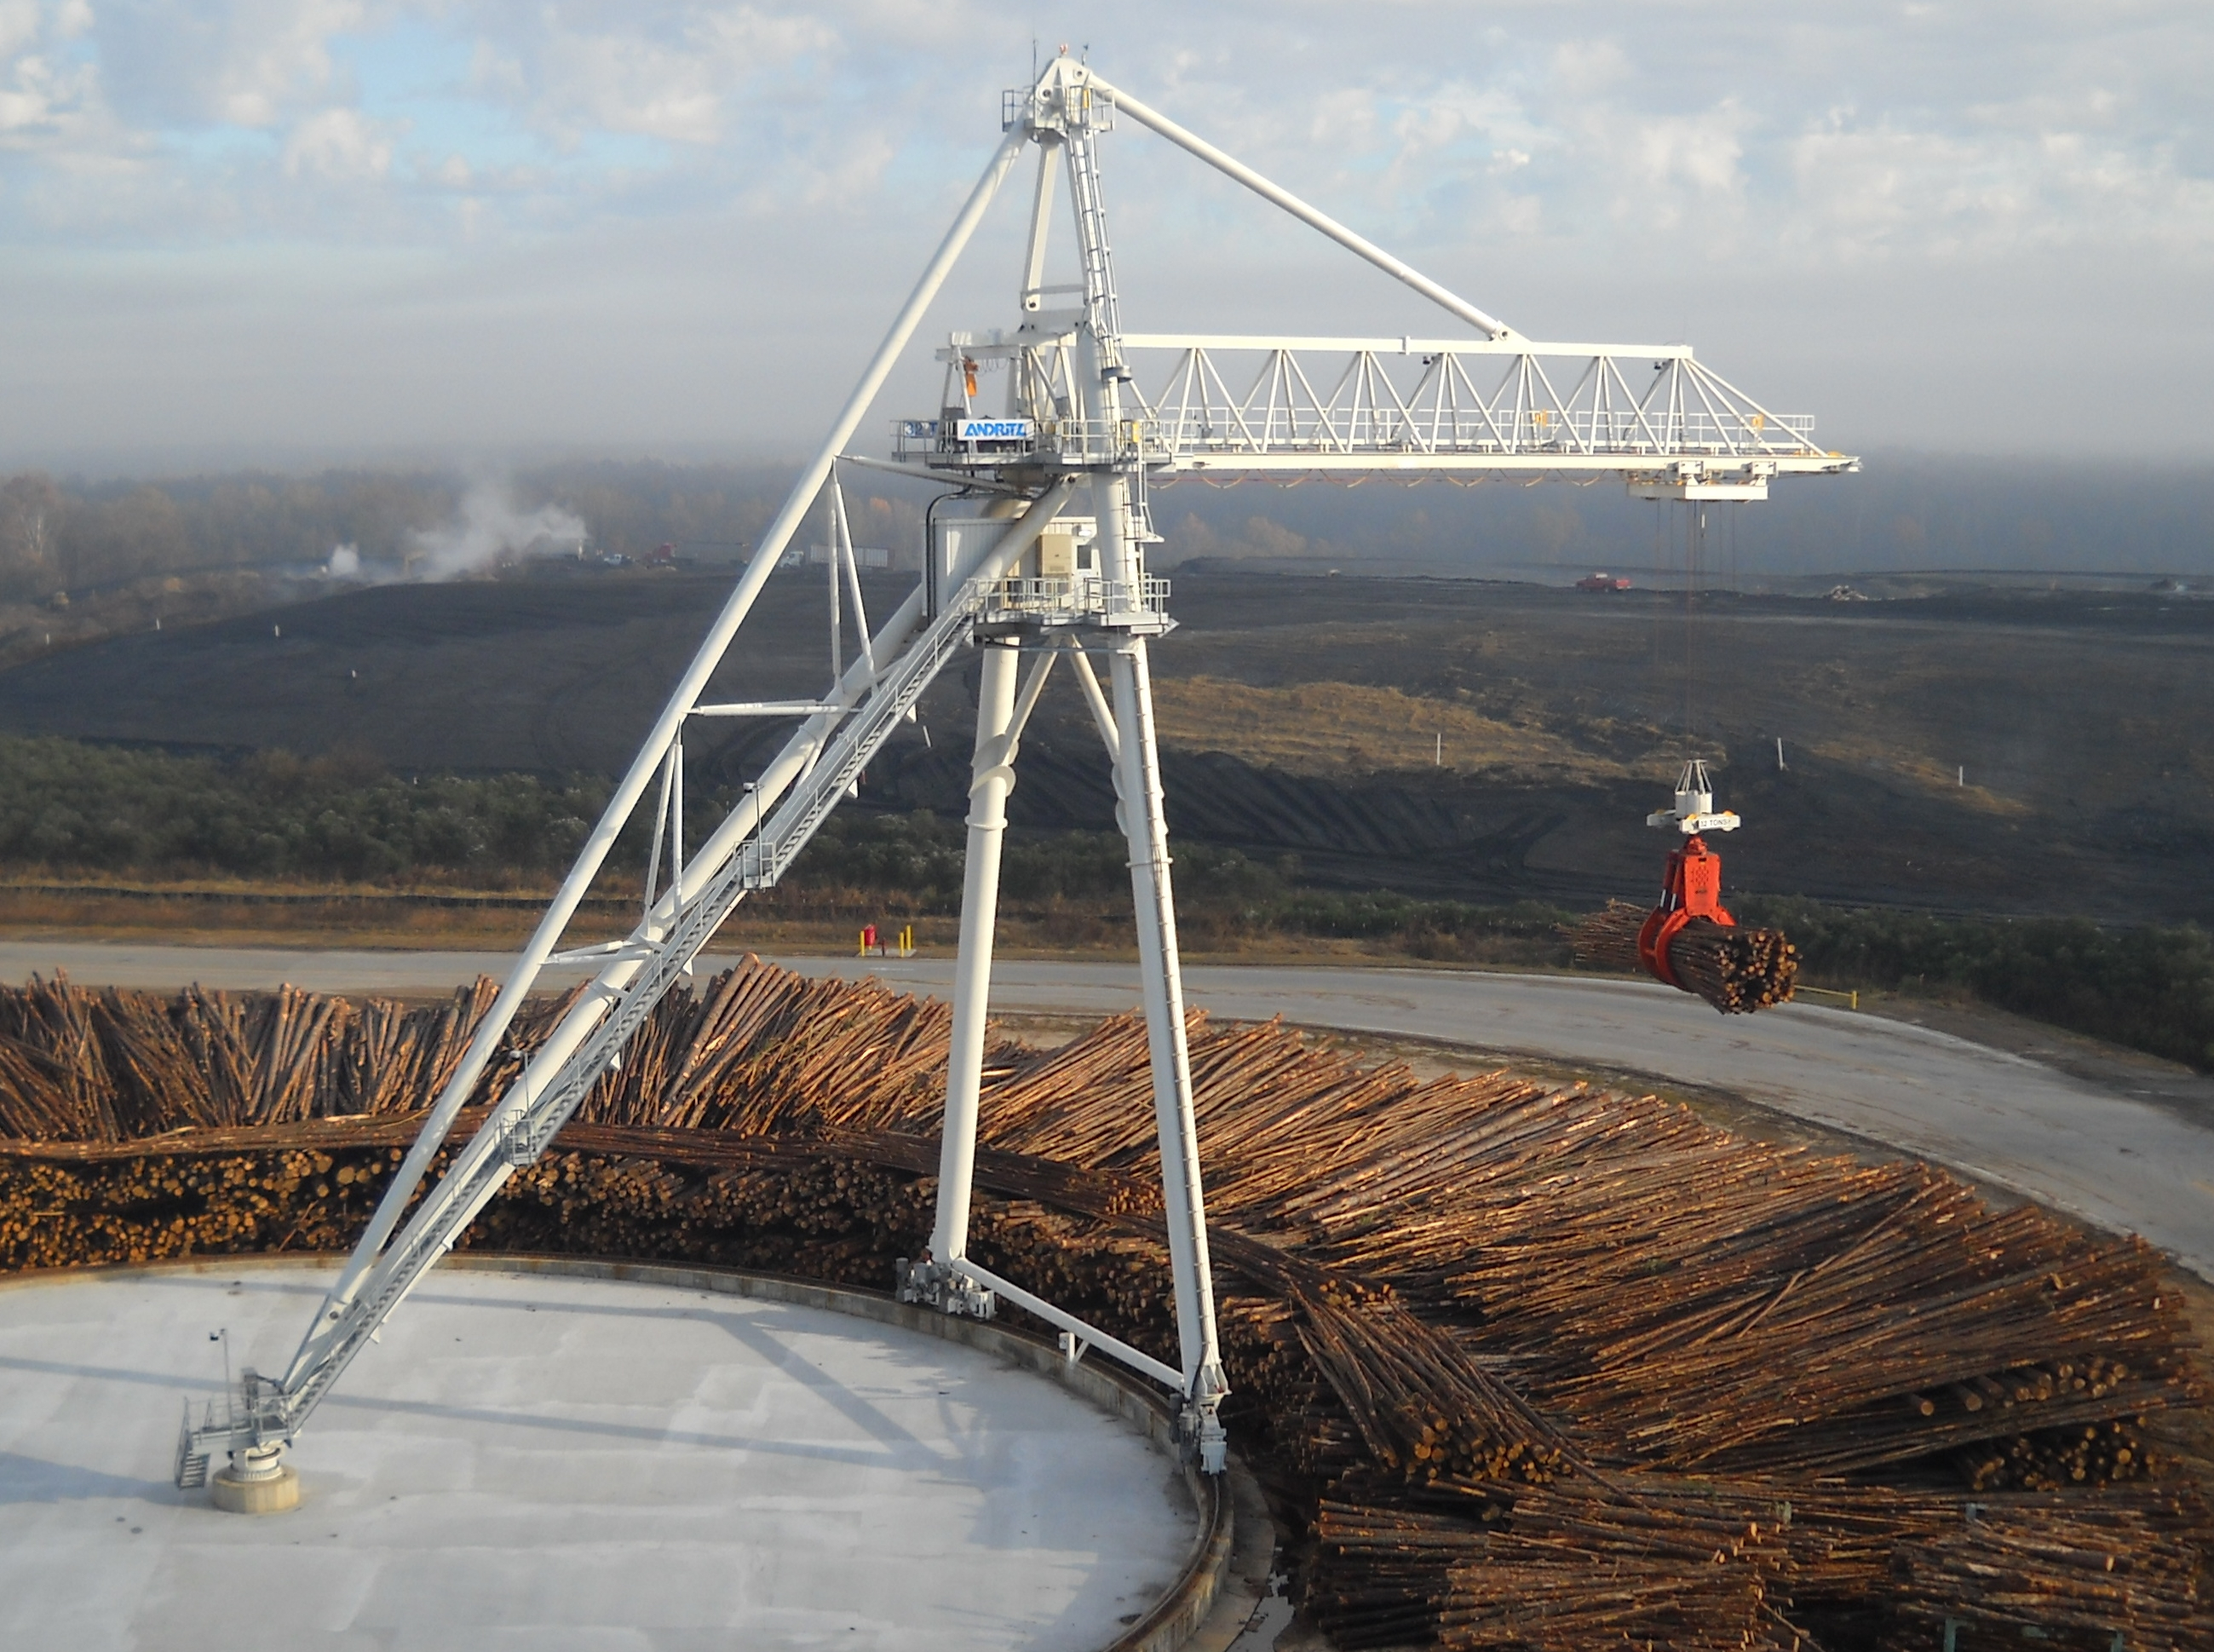
\includegraphics[width=0.5\textwidth, center]{bilder/Grundlagen/Kran_vollstaendig_N1_030.jpg}
		\caption[Rund-Kran]{Rundlaufkran (Foto: ANDRITZ)}
		\label{img:CircularCrane}
	\end{figure}		

	\paragraph{Greifer-Erkennung} 
Zur Lösung der Aufgaben wird unter anderem ein neuronales Netzwerk zur Positionserkennung des Greifers eingesetzt. Für diese Arbeit werden Vorhersagen des Netzes als Vergleichswert für die Versuche genutzt. Das Netz liegt als frozen\_inference\_graph.pb vor. Protocoll Buffer  [https://developers.google.com/protocol-buffers/] ist ein sprachneutraler, plattformneutraler, erweiterbarer Mechanismus zur Serialisierung strukturierter Daten. In diesem Fall enthält die Datei den eingefrorenen Graph und die Model Gewichte. Vorhersagen können mittels einer Tensorflowsession getroffen werden. Dabei liefert das Model, Rahmen in welchem sich der Greifer befindet 	[https://leimao.github.io/blog/Save-Load-Inference-From-TF-Frozen-Graph/]
		
	\paragraph{Baumstamm-Klassifikation} 
	Ein Klassifikatior, für die Frage ob sich Baumstämme in dem Greifer befinden liegt als meta\_graph vor. Die Vorhersage des Modells liefert die vorhergesagte Klasse mit einer Wahrscheinlichkeit zurück.

	\section{Datenverständnis}
	\label{sec:DataUnderstanding}
	Anlehnend dem in Kapitel \ref{sec:Vorgehen} beschriebenen Vorgehen \todo{Vorgehen auch so beschreiben /  ansonsten Kapitel Einleitung anpassen} werden in diesem Kapitel die zur Verfügung stehenden Daten und deren Qualität beschrieben. Dabei ist das Kapitel entsprechend der Beschriftung der Daten in zwei Teilbereiche unterteilt.
	
	Im Rahmen des Autocrane-Projektes \ref{sec:BestehendesSystem} \todo{Im Kapitel Bestehdens System erwähnen / diesen Teil in das andere Kapitel verschieben?} wurde eine Kamera an einem Rundlaufkran angebracht. Die Kamera ist so ausgerichtet, dass sich Aufhängung des Greifers am mittleren oberen Bildrand befindet. Bei einem Rundlaufkran kann die Auslenkung komplett um das Zentrum des Krans bewegt werden. Der Hintergrund der Bilder kann sich stark ändern. Mittels der Kamera werden kontinuirlich neue unbeschriftete Bilder aufgenommen und bei PSIORI abgelegt. Zu Beginn dieser Arbeit standen mehr 385.000 nicht beschriftete Bilder zur Verfügung. Die Bilder sind 1024 auf 648 Pixel groß und in Farbe. Sie sind in der Form (1024, 648, 3). Die einzelnen Pixel können dabei Werte zwischen 0 und 255 annehmen. 
	Zum Erreichen der Zielstellung werden zwei Datensätze benötigt.
	
		\paragraph{Greifer Datensatz} Der Greifer Datensatz enthält Bilder, in welchen der Greifer mittels Rahmen markiert ist. Abbildung \ref{img:Logs}  zeigt ein beispielhaftes Bild mit markiertem Greifer. Abbildung \ref{img:Grapple} zeigt ein beispielhaftes Bild mit markiertem Greifer.
		\begin{figure}[h]
				\centering
				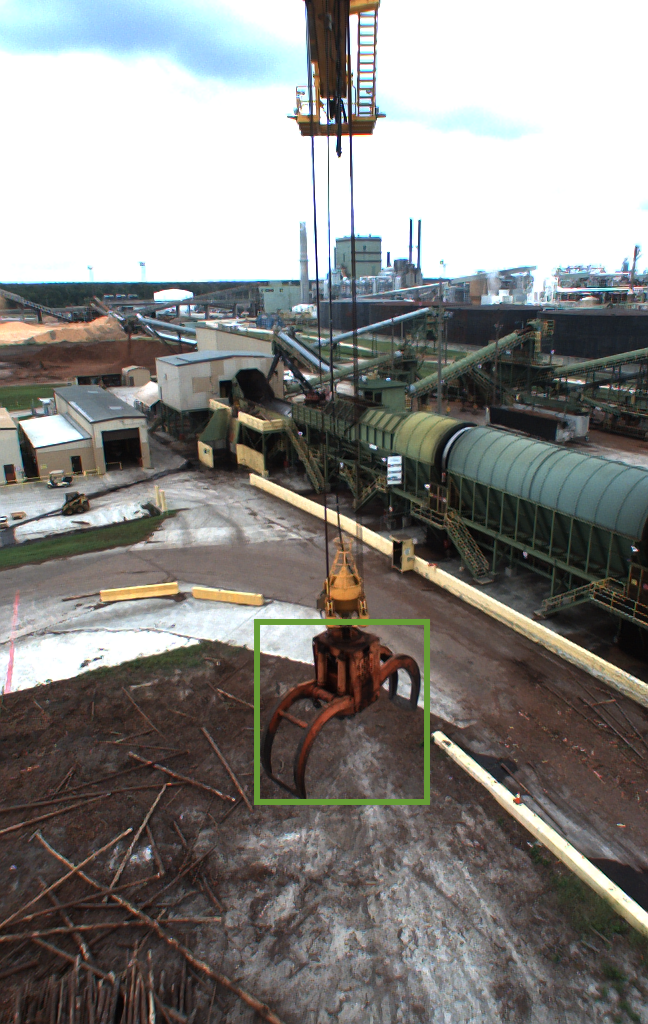
\includegraphics[width=0.5\textwidth, center]{bilder/Grundlagen/Grapple_8.png}
				\caption[Bsp. Bild: Greifer mit Rahmen]{Greifer mit Rahmen}
				\label{img:Grapple}
		\end{figure}
		Der Datensatz besteht aus zwei Sammlungen von qualitativ unterschiedlich gut beschrifteten Bildern. Die eine Sammlung besteht aus einem bestehenden Datensatz, welcher 4.684 durch Menschen annotierten Bildern enthält. Für den zweiten Teil der Sammlung wurden mittels der bestehenden Objekterkennung 14.018 Bilder annotiert. 
		
		\paragraph{Baumstamm Datensatz} Der Baumstamm Datensatz enthält Bilder, welche die Annotation, ob sich Baumstämme im Greifer befinden haben. Abbildung \ref{img:Logs} zeigt ein Bild, in welchem der Greifer Baumstämme greift. In Abbildung \ref{img:Grapple} befinden sich keine Baumstämme im Greifer.
		\begin{figure}[h]
			\centering
			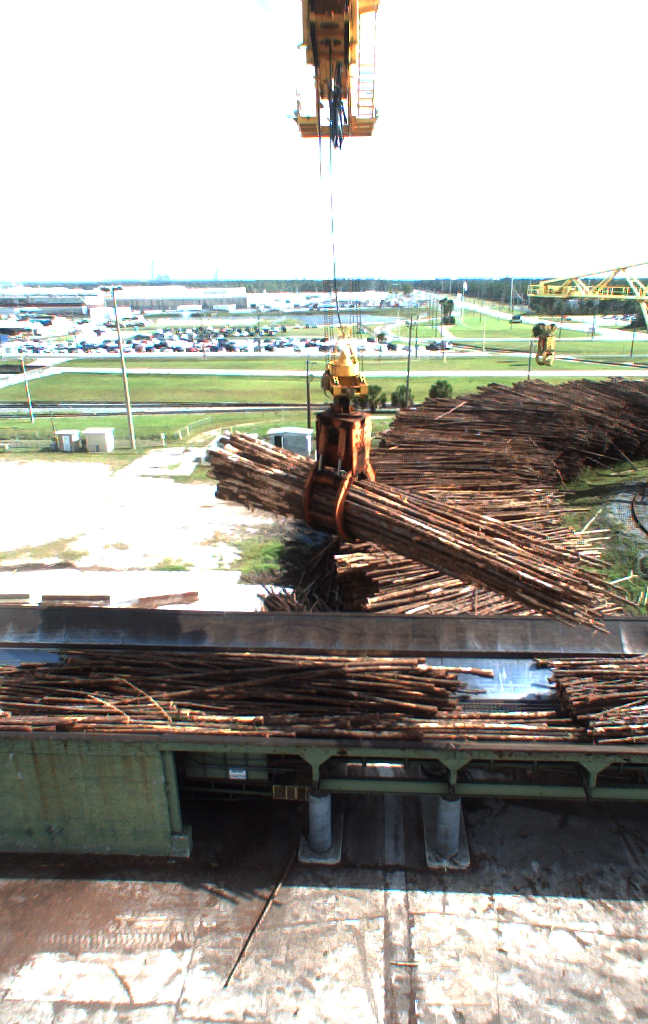
\includegraphics[width=0.5\textwidth, center]{bilder/Grundlagen/Logs_14.png}
			\caption[Bsp. Bild: Greifer mit Baumstämmen]{Greifer mit Baumstämmen}
			\label{img:Logs}
		\end{figure}
		Der Datensatz wurde im Zusammenarbeit mit quality-match[https://www.quality-match.com/imprint] und Crowdworkern erstellt.  

		\paragraph{Weiterer Datensatz}
		Im laufe der Arbeit wurden in Zusammenarbeit mit quality-match ein weiterer Datensatz erstellt. Dieser Datensatz enthält \todo{finale Zahl setzen} 80.000 beschriftete Bilder. Es wurden sowohl die Beschriftung "Logs ja / nein" als auch die Beschriftung  Rahmen des Greifers erstellt. Zusätzlich wurden weitere Beschriftungen wie Hellichkeit, Winkel des Greifers, ... erstellt. Dieses weiteren Beschriftungen wurden in der Arbeit nicht genutzt.		\todo{stimmt das am Ende noch?}
	
		
	\section{Datenvorbereitung}
	\label{sec:DataPreparation}

Die Datenvorbereitung dient dazu, einen finalen Datensatz zu erstellen, der die Basis für die nächste Phase der Modellierung bildet.


			In dem Schritt Datenvorbereitung werden die Bilder für die Modellerstelung vorbereitet. In dieser Arbeit wurde für diesen Schritt eine Klasse Preprocessing in einem neuen Modul data\_preperation.py  erstellt. Wie in Listing 
			% \lstinputlisting[language=Python,caption={Preprocessing},label=lst:Preprocessing]{\srcloc/data\_preperation.py }
			
			 zu sehen werden die Pixel der Bilder zwischen 0 und 1 Skaliert. Dei Skalierung erfolgt damit jedes Bild eine ähnliche Gewichtung
			
			Neural networks process inputs using small weight values, and inputs with large integer values can disrupt or slow down the learning process. As such it is good practice to normalize the pixel values so that each pixel value has a value between 0 and 1.
			
			Die Bilddaten werden 		
			
			\todo{Pretrain erläutern}

 

	\begin{table}[ht]
	\centering
	\begin{tabularx}{\textwidth}{lllll}
		 & \textbf{Train} & \textbf{Test}  & \textbf{Validation} & \textbf{Summe} 								  \\
		\textbf{Greifer} 				 & 	X					&	X					& 4.684 				   & x 				\\
		\textbf{Baumstämme T/F}	 	  &  X					 &	X					 &	X							& 18000		\\
		
		
		logs 5671
		not loaded 6542 
		 
		train 9.771 l 4.537  nl 5.233 80
		test 1.224 l  568 nl 655  10
		val  1.225 l 568 nl 656  10
		
	\end{tabularx}
	\caption{Datenaufteilung - Train Test Validation}
	\label{table:DatenaufteilungTrainTestValidation}
 	\end{table}
 
